\chapter{Implementation}
  The language of choice we used for the implementation is python2.7. Although we also could have implemented the extension in c/c++ since the basic version
  was already written in this language, but python does have some key benefits we did not want to miss.
  \begin{description}
    \item [Rapid prototyping]
    Since our algorithms can easily work on a given set of data completely independent and the interfaces to get the data from are clearly defined and accessible,
    using a lightweight language like python had the benefit of not having to embed our new code into the existing environment. Although it still can be implemented 
    in the native language C/C++ for our scenario, this will take some more time and effort, which was not the focus of this work.
    \item[Existing libraries]
    like NetworkX in python made it particulary easy for us to map real world scenarios to graph abstractions as we did not have to create those structures ourselves.
    Although there are some libraries that provide graph abstractions in C/C++ we could not have as easily employed them due to their copyright restrictions and 
    the closed source virtue of our target system.
    \item[Faster Debugging]
    Especially the initial phase of the project was errorprone and needed a lot of debugging. Not having to recompile after every fix turned out to be
    a great saving of time. Not to mention the live debugging capabilities of python, which was really helpful.
    \item[Existing APIs]
    Fortunately also the code for interaction with the interfaces (SNMP/SSH/Telnet) of the WLC was written in Python, so we could easily 
    integrate it into ours and had no problem gathering the 'seen'-data. Unfortunately for you those libraries are closed source to the public.
    \item[Maintainability]
    As python has the reputation of being an easy to learn language, this was another benefit and played absolutely in our favor with the goal of
    keeping the code simple, lightweight and reuseable by someone else.
  \end{description}
  \begin{figure}[t]
    \centering
    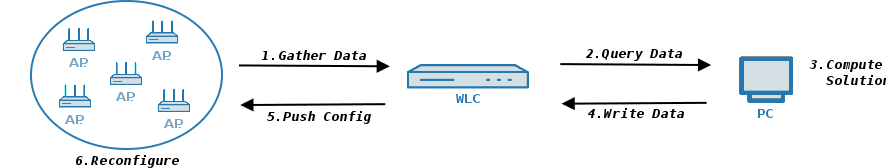
\includegraphics[width=1\columnwidth]{figures/dataflow}
    \caption{General flow of information for our scenario}
    \label{fig:dataflow}
  \end{figure}
\section{Dependencies}
  As already mentioned we used NetworkX\cite{hagberg-2008-exploring} to model our graphs and work with its elements.
  NetworkX's rich features like ``has\_path'' made things especially easy in computing the survival paths.
  Another library we used is collections. //TODO CITE collections// 
  This library implements specialized container datatypes additionally to those shipped with python already.
  It's `Counter` structure is used to create the channel-lists and retrieve the most or least used elements.
  We extended this library for our convencience since it did only provide the functionality for getting the most common element from its list and not the least common,
  which we needed. It is worth metioning that the request for including this method was already issued at 01/2013 (http://bugs.python.org/issue16994 //TODO how to cite this?),
  The only closed source library we used is the herein before mentioned library to query the WLC for the data of the APs. Nevertheless Gathering the data can also
  easily be separated and outsourced.
\section{Structure of the Code}
  Kann man den Code in gruppen einteilen, wenn ja in welche? Welche Funktionen gibt es? Was tun diese?
  \subsection{Selecting the Network Topology}
    \subsubsection{Minimal Spanning Tree}
    \subsubsection{Adding Redundand Paths}
  \subsection{Coloring the Edges/Modules}
\section{Problems}
  \begin{description}
   \item[Have there been problems with the implementation?]
   Actually no
   \item[What else could count as a problem / What else could fit in here?]
  \end{description}
\section{Run It Yourself}
  \begin{description}
   \item[What is needed to run the algorithm on your own machine?]
    Input data is required (aka which access point sees what other acces point with what Signal to Noise Ratio?) \newline
  \end{description}
